\documentclass[12pt]{article}
\usepackage[T1]{fontenc}
\usepackage{polski}
\usepackage[utf8]{inputenc}
\newcommand{\BibTeX}{{\sc Bib}\TeX} 
\usepackage{graphicx}
\usepackage{amsfonts}

\setlength{\textheight}{21cm}

\title{{\bf Zadanie nr 1 -  Sieć Kohonena do kompresji obrazów}\linebreak
Inteligentne przetwarzanie danych}
\author{Tomasz Stachura, 233264 \and Łukasz Rogoziński, 233261}
\date{16.05.2020}

\begin{document}
\clearpage\maketitle
\thispagestyle{empty}
\newpage
\setcounter{page}{1}
\section{Cel zadania}
Celem zadania była implementacja sieć neuronowej Kohonena do kompresji obrazu

\section{Wstęp teoretyczny}

\subsection{Algorytm Kohonena}
 Sieć Kohonena to samo-organizująca się mapa wykorzystująca  algorytm uczenia się bez nadzoru, używanym do zmniejszania wymiarów danych i grupowania danych. Jej struktura składa się z jednowarstwowej liniowej dwuwymiarowej siatki neuronów. Wszystkie węzły na tej siatce są podłączone tylko i wyłącznie bezpośrednio do wektora wejściowego. Oznacza, że węzły nie znają wartości swoich sąsiadów i jedynie aktualizują wagę swoich połączeń w zależności od danych wejściowych. Sama siatka jest mapą, która organizuje się przy każdej iteracji w zależności od danych wejściowych. Dobór wag neuronów jest realizowany według wzoru (1).
\begin{equation}
    w_i_j(t+1)= w_i_j(t)+\alpha_i(t)\beta_i_j[x(t)-w_i_j(t)]
\end{equation}
 Zaktualizowana waga powinna uwzględniać fakt, że efekt uczenia się jest prawie żaden na krańcach sąsiedztwa, ponieważ ilość uczenia się powinna maleć wraz z odległością. Dlatego wagi modyfikowane są z wykorzystaniem gaussowskiej funkcji sąsiedztwa βij (t), którą można zapisać:
\begin{equation}
\beta_i_j(t)=\exp\left(-\frac{d^2(i,j)}{2\sigma^2(t)}\right)
\end{equation}
gdzie $d(i,j)$ jest odległością Euklidesową pomiędzy zwycięzcą $(j)$, a i-tym
neuronem z sąsiedztwa. Odległość euklidesowa między wektorem ciężaru każdego węzła a bieżącą instancją wejściową jest obliczana na podstawie wzoru Pitagorasa.
\begin{equation}
d = min( || \overrightarrow{x} - \overrightarrow{w_i_j} || ) =min \left(\sqrt{\sum_{t=0}^{n}[\overrightarrow{x}(t) - \overrightarrow{w_i_j}(t)]^{2}}\right)
\end{equation}

\section{Eksperymenty i wyniki}

Opis wykonywanych eksperymentów. Wymagane jest ilustrowanie przeprowadzanych doświadczeń wykresami oraz tabelami.

%%%%%%%%%%%%%%%%%%%%%%%%%%%%%%%%%%%%%%%%%%%%%%%%%%%%%%%%%%%%%%%%%%%%%%%%%%%%%%%%%%%%%%%%%%%%%%%%%%%%%%%%%%%%%%%%%
% PODROZDZIA£ PT. EKSPERYMENT NR 1 
%%%%%%%%%%%%%%%%%%%%%%%%%%%%%%%%%%%%%%%%%%%%%%%%%%%%%%%%%%%%%%%%%%%%%%%%%%%%%%%%%%%%%%%%%%%%%%%%%%%%%%%%%%%%%%%%%

\subsection{Eksperyment nr 1}

Eksperyment nr 1...\\
Identycznościowa funkcja aktywacji ma postać:
\begin{equation}
 \forall\: s \in \mathbb{R}\:\:\:\: f(s) = s
 \label{równanie funkcji identycznościowej}
\end{equation}
Jak widać z definicji (\ref{równanie funkcji identycznościowej}) funkcja ta...

\subsubsection{Założenia}

\subsubsection{Przebieg}
\newpage

\subsubsection{Rezultat}

Rezultaty badañ eksperymentalnych przedstawione są w Tab. \ref{wyniki eksperymentu pierwszego}.
\begin{table}[h!]
 \caption{Rezultaty eksperymentu nr 1}
 \centering
 \vspace{0.2cm}
 \begin{tabular}{c c c c}
  \hline\hline\\[-0.4cm]
  \textbf{Przypadek} & \textbf{Metoda 1} & \textbf{Metoda 2} & \textbf{Metoda 3}\\[0.1cm]
  \hline
  \textbf{1} & 50 & 837 & 970  \\
  \textbf{2} & 47 & 877 & 230  \\
  \textbf{3} & 31 &  25 & 415  \\
  \textbf{4} & 35 & 144 & 2356 \\
  \textbf{5} & 45 & 300 & 556  \\ [0.1cm]
  \hline
 \end{tabular}
 \label{wyniki eksperymentu pierwszego}
\end{table}

\noindent Jak widać w Tab. \ref{wyniki eksperymentu pierwszego}...\newline
Graficzna interpretacja wyników z Tab. \ref{wyniki eksperymentu pierwszego} 
przedstawiona jest na wykresie Rys. \ref{rysunek do eksperymentu pierwszego} gdzie  można zauważyć że...
\begin{figure}[h!]
 \centering
 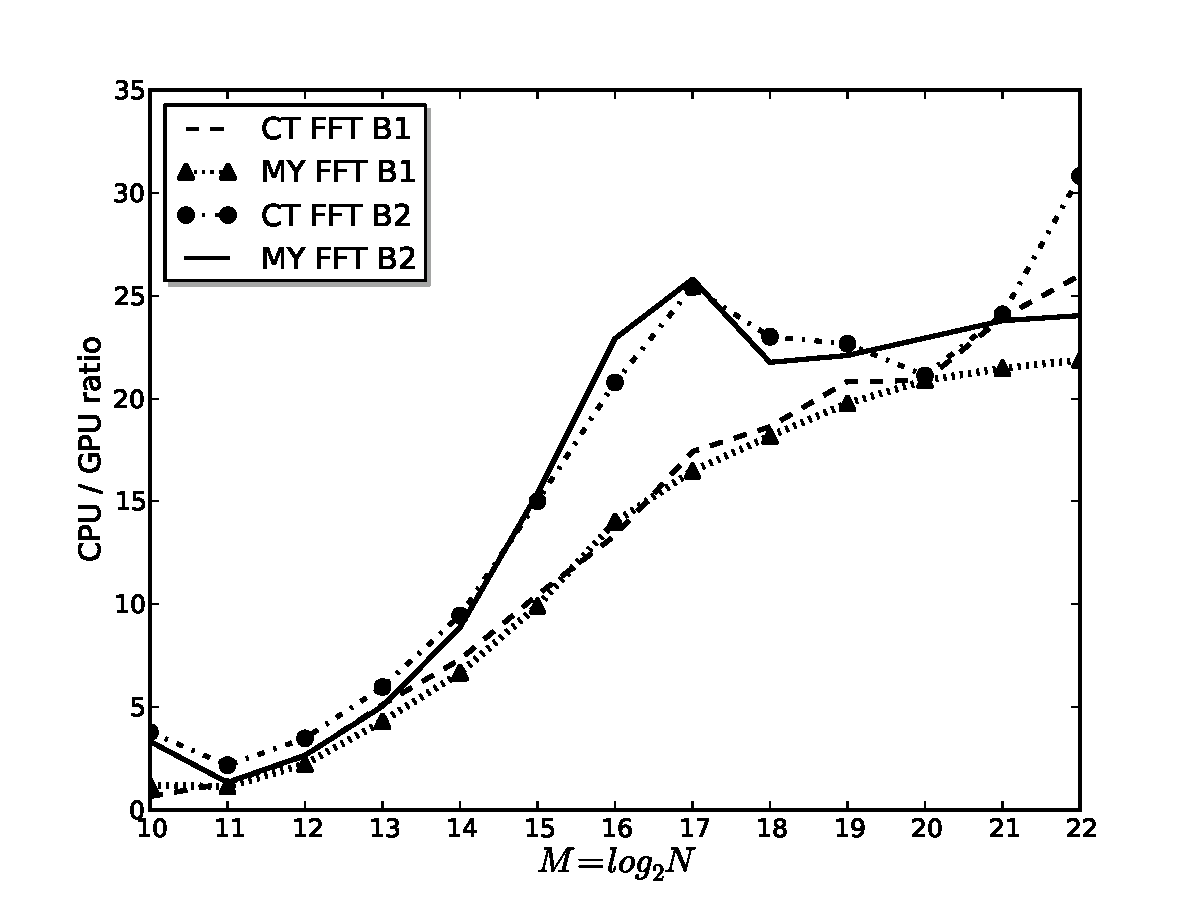
\includegraphics[width=9.3cm]{wykres.pdf}
 \vspace{-0.3cm}
 \caption{Wykres dla wyników eksperymentu pierwszego}
 \label{rysunek do eksperymentu pierwszego}
\end{figure}

\noindent Jak widać z wykresu Rys. \ref{rysunek do eksperymentu pierwszego}...\newline

%%%%%%%%%%%%%%%%%%%%%%%%%%%%%%%%%%%%%%%%%%%%%%%%%%%%%%%%%%%%%%%%%%%%%%%%%%%%%%%%%%%%%%%%%%%%%%%%%%%%%%%%%%%%%%%%%
% PODROZDZIAł PT. EKSPERYMENT NR 2 
%%%%%%%%%%%%%%%%%%%%%%%%%%%%%%%%%%%%%%%%%%%%%%%%%%%%%%%%%%%%%%%%%%%%%%%%%%%%%%%%%%%%%%%%%%%%%%%%%%%%%%%%%%%%%%%%%

\newpage
\subsection{Eksperyment nr 2}

Eksperyment nr 2 polega na...\\
Sigmoidalna funkcja aktywacji ma postać:
\begin{equation}
 \forall\: s \in \mathbb{R}\:\:\:\:\:\: f(s) = \frac{1}{\:\:\:1 + e^{-\beta \cdot s}\:}\:,
 \:\:\:\:\textnormal{gdzie}\:\:\beta \in \mathbb{R}_{+}
 \label{równanie funkcji sigmoidalnej}
\end{equation}
Jak widać z równania definicyjnego (\ref{równanie funkcji sigmoidalnej}) 
funkcja\footnote{ang. \textit{sigmoidal function} lub \textit{unipolar function}}
ta ma wykres przedstawiony 
na rysunku Rys. \ref{funkcja sigmoidalna}, gdzie parametr $\beta$ ...
\begin{figure}[h!]
 \centering
 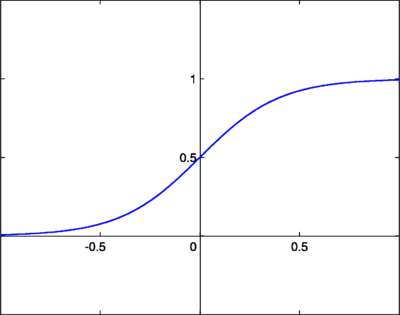
\includegraphics[width=7.3cm]{funkcja.png}
 \vspace{-0.1cm}
 \caption{Wykres funkcji sigmoidalnej}
 \label{funkcja sigmoidalna}
\end{figure}

\subsubsection{Założenia}

\subsubsection{Przebieg}

\subsubsection{Rezultat}

Rezultaty badań eksperymentalnych przedstawione są w Tab. \ref{wyniki eksperymentu drugiego}.
\vspace{-0.5cm}
\begin{table}[h!]
 \caption{Rezultaty eksperymentu nr 2}
 \centering
 \vspace{0.2cm}
 \begin{tabular}{c c c }
  \hline\hline\\[-0.4cm]
  \textbf{Przypadek} & \textbf{Metoda 1} & \textbf{Metoda 2}\\[0.1cm]
  \hline
  \textbf{1} & 50 & 837 \\
  \textbf{2} & 47 & 877 \\
  \textbf{3} & 45 & 300 \\ [0.1cm]
  \hline
 \end{tabular}
 \label{wyniki eksperymentu drugiego}
\end{table}

\noindent Jak widać w Tab. \ref{wyniki eksperymentu drugiego}...\newline
Wyniki w Tab. \ref{wyniki eksperymentu drugiego} świadczą o tym, że...

%%%%%%%%%%%%%%%%%%%%%%%%%%%%%%%%%%%%%%%%%%%%%%%%%%%%%%%%%%%%%%%%%%%%%%%%%%%%%%%%%%%%%%%%%%%%%%%%%%%%%%%%%%%%%%%%%
% PODROZDZIA£ PT. EKSPERYMENT NR N 
%%%%%%%%%%%%%%%%%%%%%%%%%%%%%%%%%%%%%%%%%%%%%%%%%%%%%%%%%%%%%%%%%%%%%%%%%%%%%%%%%%%%%%%%%%%%%%%%%%%%%%%%%%%%%%%%%

\subsection{Eksperyment nr n}
Eksperyment nr zakłada iż...\\
Dla dowolnej liczby $N \in \mathbb{N}$ funkcjê 
$F_{N}:\mathbb{C}^{\:N}\!\rightarrow\mathbb{C}^{\:N}$
zdefiniowana w następujący sposób:
\vspace{-0.4cm}
\begin{equation}
 \forall\:\mathbf{x} \in \mathbb{C}^{\:N}\:\:\:\:\:
 \forall\:k \in \{\:0,\dots,N - 1\:\!\}\:\:\:\:\:
 F_{N}\:\!(\:\mathbf{x}\:)_{k}\:\stackrel{\Delta}{=}\:
 \frac{1}{\sqrt{N}}\:
 \sum_{n = 0}^{N - 1}\:x_{n}\:\cdot\:
 e^{-j 2 \pi n k / N}
 \label{równanie dyskretnej transformaty Fouriera}
\end{equation}
nazywamy $N$ -- punktowym prostym jednowymiarowym dyskretnym przekształceniem Fouriera.
Na Rys. \ref{FFT} przedstawiono szybki algorytm obliczania dyskretnego 
przekształcenia Fouriera\footnote{ang. \textit{Fast Fourier Transform}}.
\begin{figure}[h!]
 \centering
 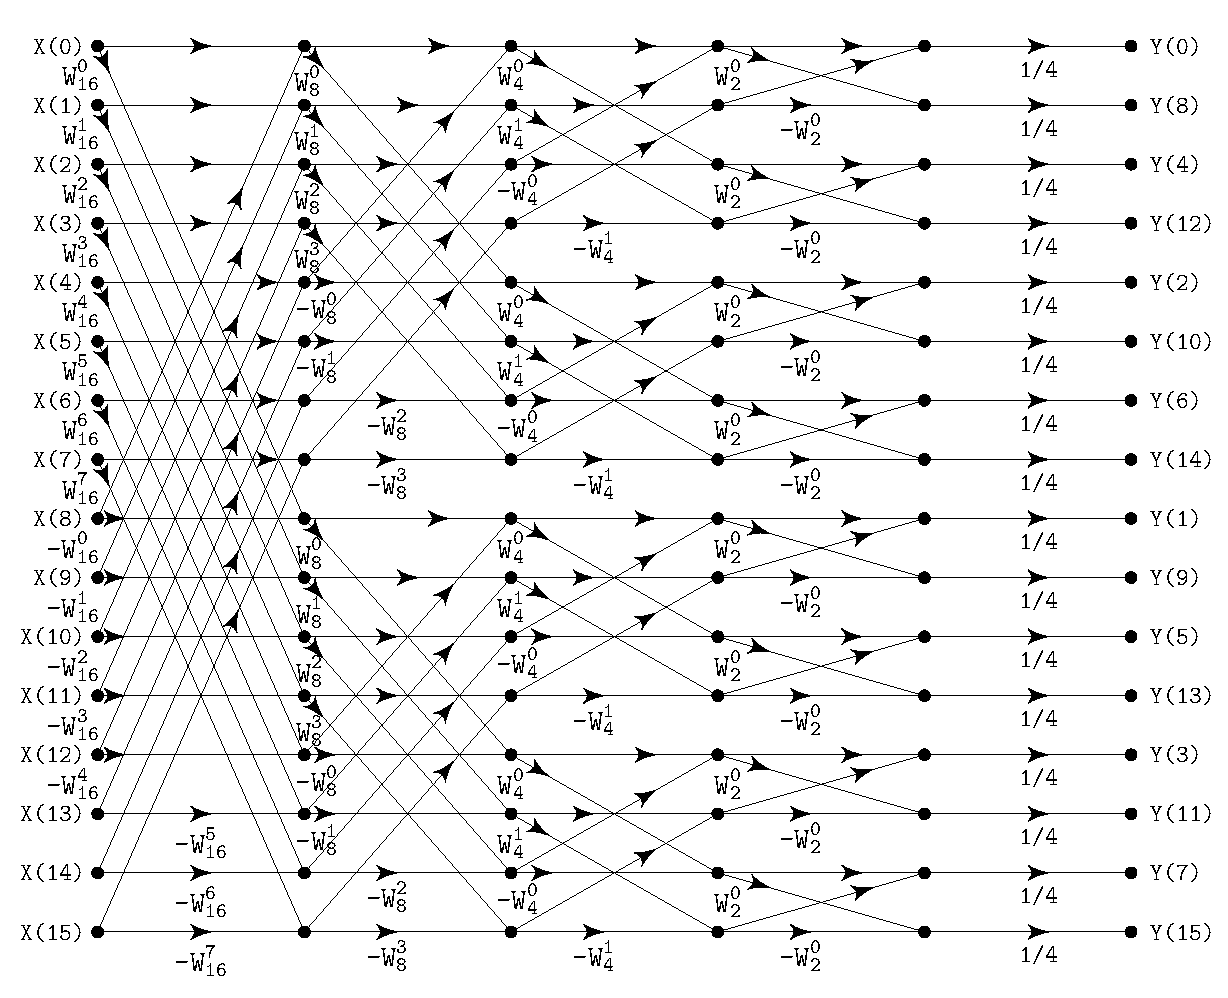
\includegraphics[width=0.8\linewidth]{transformata.pdf}
 \vspace{-0.1cm}
 \caption{Szybkie przekształcenie Fouriera}
 \label{FFT}
\end{figure}

\subsubsection{Założenia}

\subsubsection{Przebieg}

\subsubsection{Rezultat}
\newpage

\section{Wnioski}

Wnioski z przeprowadzonych eksperymentów dowodzi, że...


%%%%%%%%%%%%%%%%%%%%%%%%%%%%%%%%%%%%%%%%%%%%%%%%%%%%%%%%%%%%%%%%%%%%%%%%%%%%%%%%%%%%%%%%%%%%%%%%%%%%%%%%%%%%%%%%%
% PODROZDZIA£ PT. ZAŁĄCZNIKI
%%%%%%%%%%%%%%%%%%%%%%%%%%%%%%%%%%%%%%%%%%%%%%%%%%%%%%%%%%%%%%%%%%%%%%%%%%%%%%%%%%%%%%%%%%%%%%%%%%%%%%%%%%%%%%%%%

\section{Załączniki}

Opcjonalnie, w załączniki od zadania,
np. fragment kodu źródłowego.


%%%%%%%%%%%%%%%%%%%%%%%%%%%%%%%%%%%%%%%%%%%%%%%%%%%%%%%%%%%%%%%%%%%%%%%%%%%%%%%%%%%%%%%%%%%%%%%%%%%%%%%%%%%%%%%%%
% BIBLIOGRAFIA
%%%%%%%%%%%%%%%%%%%%%%%%%%%%%%%%%%%%%%%%%%%%%%%%%%%%%%%%%%%%%%%%%%%%%%%%%%%%%%%%%%%%%%%%%%%%%%%%%%%%%%%%%%%%%%%%%

\renewcommand\refname{Bibliografia}
\bibliographystyle{plain}
\begin{thebibliography}{0}
\bibitem{l2short} T. Oetiker, H. Partl, I. Hyna, E. Schlegl.
\textsl{Nie za krótkie wprowadzenie do systemu \LaTeX2e}, 2007, dostępny online.
\bibitem{12short} T. Kohonen.
\textsl{Self-organising Maps. Springer, Berlin - Heidelberg}1995.
\bibitem{12short} E. Skubalska-Rafajłowicz, M. Nałęcz.
\textsl{Samo-organizujące sieci neuronowe. Biocybernetyka i Inżynieria Biomedyczna }2000, Tom 6: Sieci neuronowe, str. 187–188
\bibitem{12short}M. Krętowska
\textsl{Katedra Oprogramowania, Wykład 11: Sieci samo organizujące się} 2011, Białystok, Katedra Oprogramowania.
\end{thebibliography}

\end{document}
